% Makros zur Kompatibilitaet mit Onlinemodul: 
 \providecommand{\MoIl}{(} 
 \providecommand{\MoIr}{)}
 \providecommand{\MIntvlSep}{;} 
 \providecommand{\MElSetSep}{;} 
 \begin{MAufgabe}{Kurvendiskussion}{kr, MaTeX}
 F\"uhren Sie f\"ur die Funktion $f(x)=3\, x^4 + 24\, x^3 - 162\, x^2 - 1680\, x - 8$ eine vollst\"andige Kurvendiskussion durch.\\ 
 \ifLsg\Loesung
 \begin{enumerate}
 \item \emph{Definitionsbereich:} 
 Der maximale Definitionsbereich ist $\R$\item \emph{Symmetrie:} 
 Keine Symmetrie bez\"uglich y-Achse oder Koordinatenursprung.\item \emph{Asymptotisches Verhalten:} 
 Grenzwerte f\"ur $x\rightarrow \pm \infty$: \\ 
 $\lim_{x\rightarrow \infty} f(x)=\infty$ \\ 
 $\lim_{x\rightarrow -\infty} f(x)=\infty$ \\ 
 \item \emph{Periodizit\"at:} 
 Die Funktion $f$ ist als rationale (nicht konstante) Funktion nicht periodisch.\item \emph{Ableitungen:} 
 Als rationale Funktion ist $f$ auf ihrem Definitionsbereich unendlich oft differenzierbar. 
 Die ersten 2 Ableitungen von $f$ lauten: \\ 
 $f^{(1)}(x)=12\, x^3 + 72\, x^2 - 324\, x - 1680$\newline 
  $f^{(2)}(x)=36\, x^2 + 144\, x - 324$\newline 
  \item \emph{Extremstellen:} 
 Eine Notwendige Bedingung f"ur Extremstellen von $f$ ist $f^{(1)}(x)=0$. 
 Das ist hier \"aquivalent zu $12\, x^3 + 72\, x^2 - 324\, x - 1680=0$. 
 Die Kandidaten f\"ur Extremstellen sind die L\"osung dieser Gleichung innerhalb des Definitionsbereichs von $f$: $-7$; $-4$; $5$; \\ 
 $f^{(2)}(-7)=432$$>0$, Minimum bei $(-7;2785)$; \\ 
 $f^{(2)}(-4)=-324$$<0$, Maximum bei $(-4;3352)$; \\ 
 $f^{(2)}(5)=1296$$>0$, Minimum bei $(5;-7583)$; \\ 
 \item \emph{Monotonieverhalten:} 
 Bei einer stetigen ersten Ableitung ist allgemein das Vorzeichen der ersten Ableitung auf Intervallen, die durch die Extremstellen und die Definitionsl\"ucken gegeben sind zu betrachten.Somit ist $f$ auf \\ 
 $\MoIl-\infty\MIntvlSep-7\MoIr$ monoton fallend, \\ 
 $\MoIl-7\MIntvlSep-4\MoIr$ monoton  wachsend, \\ 
 $\MoIl-4\MIntvlSep5\MoIr$ monoton  fallend, \\ 
 $\MoIl5\MIntvlSep \infty\MoIr$ monoton wachsend. \\ 
 \item \emph{Wendestellen:} 
 Eine Notwendige Bedingung f"ur Wendestellen von $f$ ist $f^{(2)}(x)=0$. 
 Das ist hier \"aquivalent zu $36\, x^2 + 144\, x - 324=0$. 
 Die Kandidaten f\"ur Wendestellen sind die L\"osung dieser Gleichung innerhalb des Definitionsbereichs von $f$: $ - \sqrt{13} - 2$; $\sqrt{13} - 2$; \\ 
 Wendestelle bei $( - \sqrt{13} - 2\MIntvlSep3\, {\left(\sqrt{13} + 2\right)}^4 - 24\, {\left(\sqrt{13} + 2\right)}^3 - 162\, {\left(\sqrt{13} + 2\right)}^2 + 1680\, \sqrt{13} + 3352)$, weil die zweite Ableitung das Vorzeichen von + nach - wechselt. \\ 
 Wendestelle bei $(\sqrt{13} - 2\MIntvlSep24\, {\left(\sqrt{13} - 2\right)}^3 - 162\, {\left(\sqrt{13} - 2\right)}^2 + 3\, {\left(\sqrt{13} - 2\right)}^4 - 1680\, \sqrt{13} + 3352)$, weil die zweite Ableitung das Vorzeichen von - nach + wechselt. \\ 
 \item \emph{Kr\"ummungsverhalten:} 
 Bei einer stetigen zweiten Ableitung ist allgemein das Vorzeichen der zweiten Ableitung auf Intervallen, die durch die Nullstellen der zweiten Ableitung und die Definitionsl\"ucken gegeben sind zu betrachten. 
 Somit ist $f$ auf \\ 
 $\MoIl-\infty \MIntvlSep - \sqrt{13} - 2\MoIr$  konvex ($f^{(2)}>0$), \\ 
 $\MoIl - \sqrt{13} - 2\MIntvlSep\sqrt{13} - 2\MoIr$  konkav ($f^{(2)}>0$), \\ 
 $\MoIl\sqrt{13} - 2\MIntvlSep \infty\MoIr$  konvex ($f^{(2)}>0$). \\ 
 \item \emph{Skizze des Graphen:} \\ 
 {\textcolor{red} x}: Maxima; {\textcolor{black} x}: Minima; {\textcolor{green} o}: Wendestellen; 
  \begin{center}
  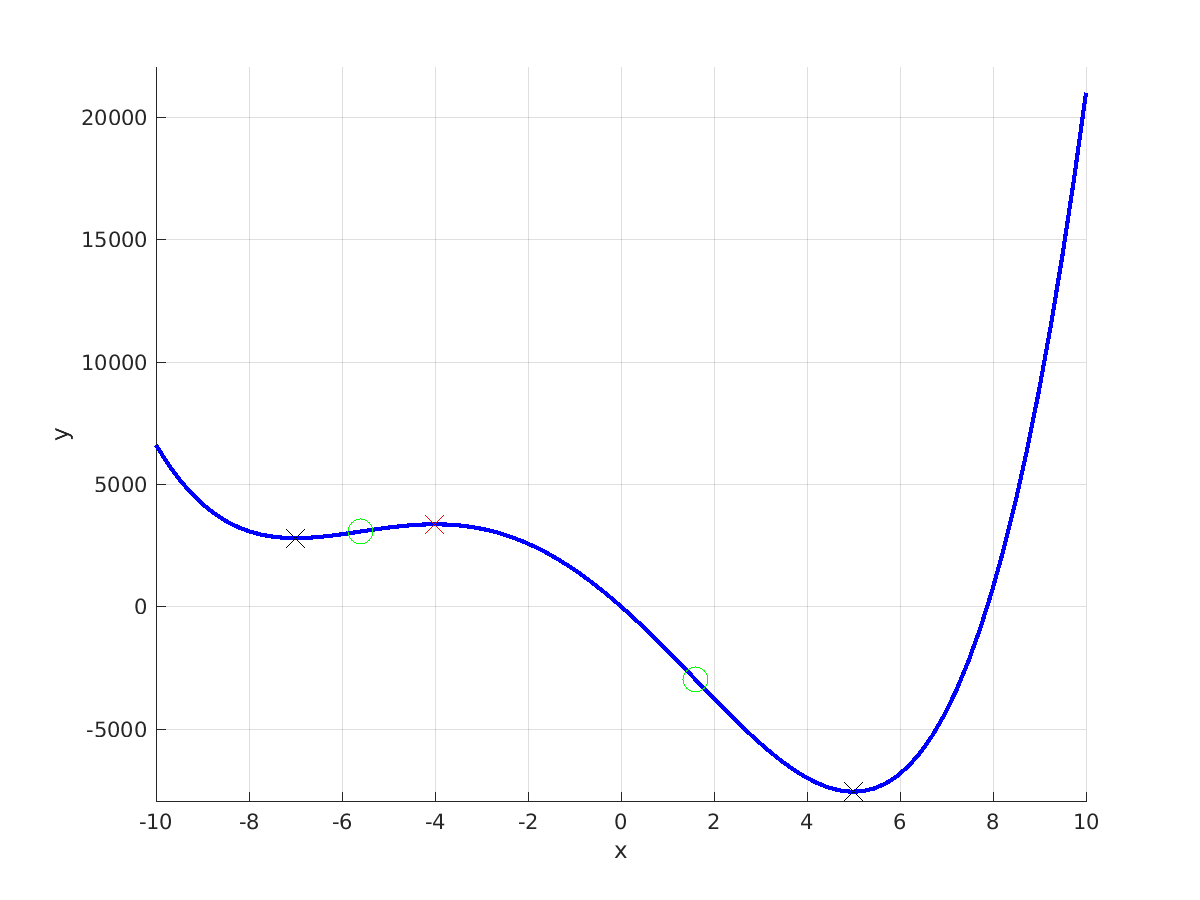
\includegraphics[width=0.8\linewidth]{Abb_zur_Ag_autogenerated_curves_8.png} \end{center}
  
 \end{enumerate}
 \else\relax\fi
  \end{MAufgabe}